\begin{figure}[t!]
\centering
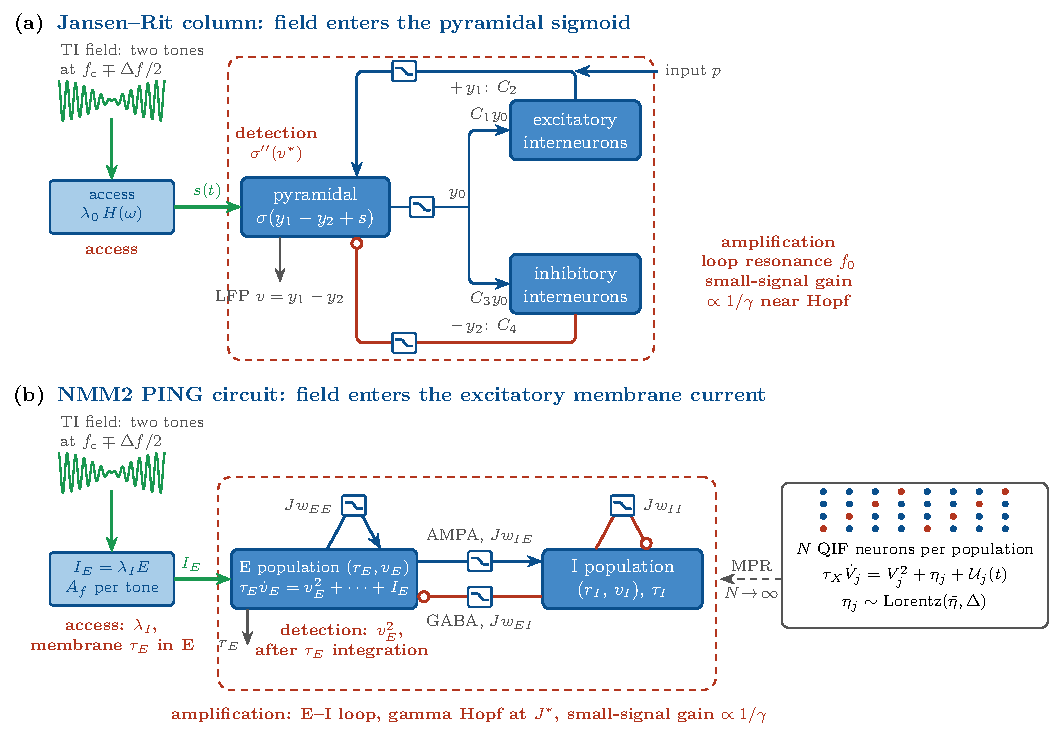
\includegraphics[width=\textwidth]{fig_models_ti.pdf}
\caption{\textbf{Access, detection, and amplification in the two circuits.}
\emph{(a)} JR: access, coupling $\lambda_0$ times filter $H(\omega)$, converts the field to polarization
$s$, and sigmoid curvature mixes the tones.
\emph{(b)} NMM2 PING: current $I_E=\lambda_I E$ (field $E$, coupling $\lambda_I$) enters the excitatory membrane;
$v_E^2$, the squared mean voltage, mixes its excursions. The inset shows the QIF neurons whose
infinite-population limit gives this exact mean field.
Low-pass symbols mark second-order synapses ($h_e,h_i$ in a; AMPA and GABA
with times $\tau_a,\tau_g$ in b). They suppress carriers more strongly than
the generated beat and transmit the steady shift.
Dashed frames enclose recurrent amplifiers, with small-signal gain
proportional to inverse modal damping $1/\gamma$ near the relevant Hopf.
Blue: excitation; red: inhibition; green: field input.}
\label{fig:models}
\end{figure}
